\documentclass{scrartcl}

% character information for fonts (needed by tipa).
\usepackage[T3,OT2,T1]{fontenc}

% package for the pretty tables
\usepackage{booktabs}

% document metadata
\author{Johannes Englisch}
\title{An Example Document}
\date{\today}

% localisation support
%  * adds support for English (US), English (UK), Russian, and German (new orthography)
%  * the *last* langauge is considered the main language for the document
\usepackage[english,british,russian,ngerman]{babel}

% set custom page margins if needed
\usepackage{geometry}
\geometry{%
  % I don't remember why includehead and includefoot are needed.
  includehead,includefoot,%
  top=2cm,bottom=2cm,%
  left=2cm,right=2cm,%
}

% turn references into hyperlinks
\usepackage{hyperref}
% metadata for the pdf
\hypersetup{
  pdftitle=Example document,
  pdfauthor=Me,
  % This line removes the annoying boxes around the links that show up in the
  % pdf.
  pdfborderstyle={/S/U/W 0},
}

% this package allows you to insert images into your document.
\usepackage{graphicx}

% bibliography package
\usepackage{natbib}
% a style I made for myself using `latex makebst`
\bibliographystyle{bibstyle-en}
% define punctuation, e.g. (cf. Miller 2022; Smith 2023a: 1–3)
\bibpunct[:\,]{\char40{}}{\char41{}}{;}{a}{}{,}
% don't automatically add a section header to the list of references.
\let\oldbibsection\bibsection{}
\renewcommand{\bibsection}{}

% linguistic examples and glosses (load last)
\usepackage{gb4e}

% ipa symbols (load even laster)
\usepackage[noenc]{tipa}

\begin{document}

% Put in the title based on the meta data from the preamble.
\maketitle

% Insert table of contents.
\tableofcontents

\section{Introduction}

This file basically functions as a~cheat sheet for common tasks and techniques
you might want to do in \LaTeX.
Note that this contains more than we could cover in the session.
Specifically, this also contains a~small bibliography, so you have to tell your
editor to run Bib\TeX{}.

\section{Paragraphs and comments}

Hello, world!
Blah blah blah.
Blah blah blah.
Blah blah blah.
Blah blah blah.
Blah blah.
% tilde ~ = non-breaking space
See Section~\ref{sec:thesubsection} at page~\pageref{sec:thesubsection}.

Second paragraph.
Third paragraph (not).
every
word
on
a
separate
line. \\
A whole sentence on a line in its entirety.

% This is a comment.  It will not show up in the pdfdocument
% btw, a comment also remove the line-break (or rather, the invisible
% end-of-line character).
this%
is%
a%
    very%
  long%
word

\section{Section headers}

\subsection{A section of a section}

\subsection*{A section without a number}

\subsubsection{Sub sub section}%
\label{sec:thesubsection}

\paragraph{Paragraph}

\section{Third section}

This is a URL:
\url{www.example.com}

\section{Formatting}

You can make text \textit{italic}, \textbf{bold-face}, \texttt{fixed-width},
\textsf{sans-serif}, \textsc{Small Caps}.

This is \emph{emphasised \emph{(really)} text}!

\section{Lists}

\begin{itemize}
  \item This an item.
  \item This is also an item.
    \begin{itemize}
      \item One
      \item Two
      \item[$\to$] Three
    \end{itemize}
\end{itemize}

\begin{enumerate}
  \item first
  \item\label{bp:second} second
  \item third
    \begin{enumerate}
      \item first
      \item\label{bp:bla} second
      \item third
    \end{enumerate}
\end{enumerate}

See element~\ref{bp:second} and~\ref{bp:bla}.

\section{Maths}

Use dollar signs for in-line maths:
$ x_i = y_i^2 + y^{(x - 1)} + 5 $ and $\sum_{i = 0}^k x_i$ are formulas.

\[
  \sum_{i = 0}^k x_i
\]

\begin{itemize}
  \item Super/subscripts: $x^2$, $x_i$, $x_i^2$, $x^{(1 - y)}$
  \item Greek letters: $\alpha = \beta + \gamma^\delta$ (don't use them to write
    actual Greek; use \texttt{\textbackslash{}selectlanguage} instead).
\end{itemize}

\subsection*{Further reading}
\begin{itemize}
  \item \url{https://en.wikibooks.org/wiki/LaTeX/Mathematics}
\end{itemize}

\section{Escaping special characters}

Characters reserved by the \TeX{} language:
\textbackslash, \{, \}, \%, \$, \_

Some non-English latin characters: \\
äöüß  \ae, \aa, \o, \l, \ss

\textipa{DIs Iz @n IgzA:mpl}

Also:
\begin{itemize}
  \item \LaTeX{} provides some easy-to-type short hands for special characters.
    There's `single quotes', ``double quotes'', or those <<\,French quotes\,>>.
  \item Also, you can make nice-looking dashes -- if you are so inclined.
    Some people---mostly Americans---also like those super-long dashes.
\end{itemize}

\subsection*{Further reading}
\begin{itemize}
  \item The Comprehensive \LaTeX{} Symbol List (a.\,k.\,a.\ \texttt{symbols-a4.pdf}): \\
    \url{https://www.ctan.org/tex-archive/info/symbols/comprehensive/}
  \item The \texttt{tipa} manual: \\
    \url{http://mirrors.ctan.org/fonts/tipa/tipa/doc/tipaman.pdf}
\end{itemize}

\section{Examples}

\begin{exe}
  \ex This is an example
  \ex[*]{\label{ex:thing}This is example a bla}
  \ex[]{This is example a bla}
  \begin{xlist}
    \ex\label{ex:otherthing} one
    \ex two
  \end{xlist}
\end{exe}

See~(\ref{ex:thing}) and~(\ref{ex:otherthing}).

Examples with glosses:

\begin{exe}
  \ex \gll Dieses Beispiel hat zwei Zeilen \\
    this example has two lines \\
    \trans `This example has two lines'
  \ex \glll Dieses Beispiel hat drei Zeilen \\
    \textipa{di:z@s} \textipa{baISpi:l} \textipa{hat} \textipa{dKaI} \textipa{tsaIln} \\
    this example has three lines \\
    \trans `This example has three lines'
  \ex \gll If things don't line up then you can {} make them! \\
    If things {do not} line up {} you can easily make them! \\
    \trans `See?'
\end{exe}

\subsection*{Further reading}
\begin{itemize}
  \item Manual of the \texttt{gb4e}: \\
    \url{http://mirrors.ctan.org/macros/latex/contrib/gb4e/gb4e-doc.pdf}
  \item \texttt{linguex} (an alternative package): \\
    \url{https://www.ctan.org/pkg/linguex}
  \item \texttt{covington} (yet another alternative): \\
    \url{https://www.ctan.org/pkg/covington}
\end{itemize}

\section{Spaces}

Some argument-less commands like \LaTeX consume the space after it.
You can avoid this problem by either adding curly braces behind the \LaTeX{}
command, around the {\LaTeX} command or by escaping the space after the
\LaTeX\ command with a backslash.
Some commands don't consume the space but I can never remember, which, so I just
put all the curly braces everwhere.

Also, \texttt{\textbackslash,} creates a~thin space, which is useful for stuff
like abbreviations or units of measurements (e.\,g.\ 1.5\,kg)

\section{Localisation}

The \texttt{babel} package add support for multi-language text.

\begin{itemize}
  \item {\selectlanguage{ngerman}Hey! Heute ist der \today!}
  \item {\selectlanguage{english}Hey! Today is \today!}
  \item {\selectlanguage{british}Hey! Today is \today!}
  \item {\selectlanguage{russian}Сегодня --- \today!}
    (You can't type Cyrillic without this\dots)
\end{itemize}

\subsection*{Further reading}

\begin{itemize}
  \item The \texttt{babel} user guide: \\
    \url{http://mirrors.ctan.org/macros/latex/required/babel/base/babel.pdf}
\end{itemize}

\section{Tables}

% naked table
\begin{center}
  \begin{tabular}{lrl}
    line 1 & line 1, again & also line 1 \\
    another line & whoop-di-do & yay \\
    foo & bar & baz \\
    is what & programmers & say \\
  \end{tabular}
\end{center}

% table with lines
\begin{center}
  \begin{tabular}{|l|r|l|}
    \hline
    line 1 & line 1, again & also line 1 \\
    \hline
    another line & whoop-di-do & yay \\
    \hline
    foo & bar & baz \\
    \hline
    is what & programmers & say \\
    \hline
  \end{tabular}
\end{center}

% typographically more pleasing table.
\begin{center}
  \begin{tabular}{lrl}
    \toprule
    line 1 & line 1, again & also line 1 \\
    \midrule
    another line & whoop-di-do & yay \\
    foo & bar & baz \\
    is what & programmers & say \\
    \bottomrule
  \end{tabular}
\end{center}

\begin{table}[h]
  % \centering is the switch version of \begin{center}...\end{center}
  \centering%
  \begin{tabular}{lrl}
    \toprule
    line 1 & line 1, again & also line 1 \\
    \midrule
    another line & whoop-di-do & yay \\
    foo & bar & baz \\
    is what & programmers & say \\
    \bottomrule
  \end{tabular}
  \caption{This is a~floating table.  \LaTeX{} will decide where to put it.}
  \label{tab:my-table}
\end{table}

Table~\ref{tab:my-table} is a~floating table.
That means \LaTeX{} will ultimately decide where it will end up in your
document.

\begin{itemize}
  \item If you say \texttt{[t]} it puts it at the top of a~page.
  \item If you say \texttt{[b]} it puts it at the bottom of a~page.
  \item If you say \texttt{[h]} it puts it \emph{somewhere here}\texttrademark.
\end{itemize}

It's recommended to avoid language like \emph{see the following table} or
\emph{see the table above}.
Instead point to your table using a~cross reference.

\section{Images and figures}

\begin{figure}[h]
  \centering%
  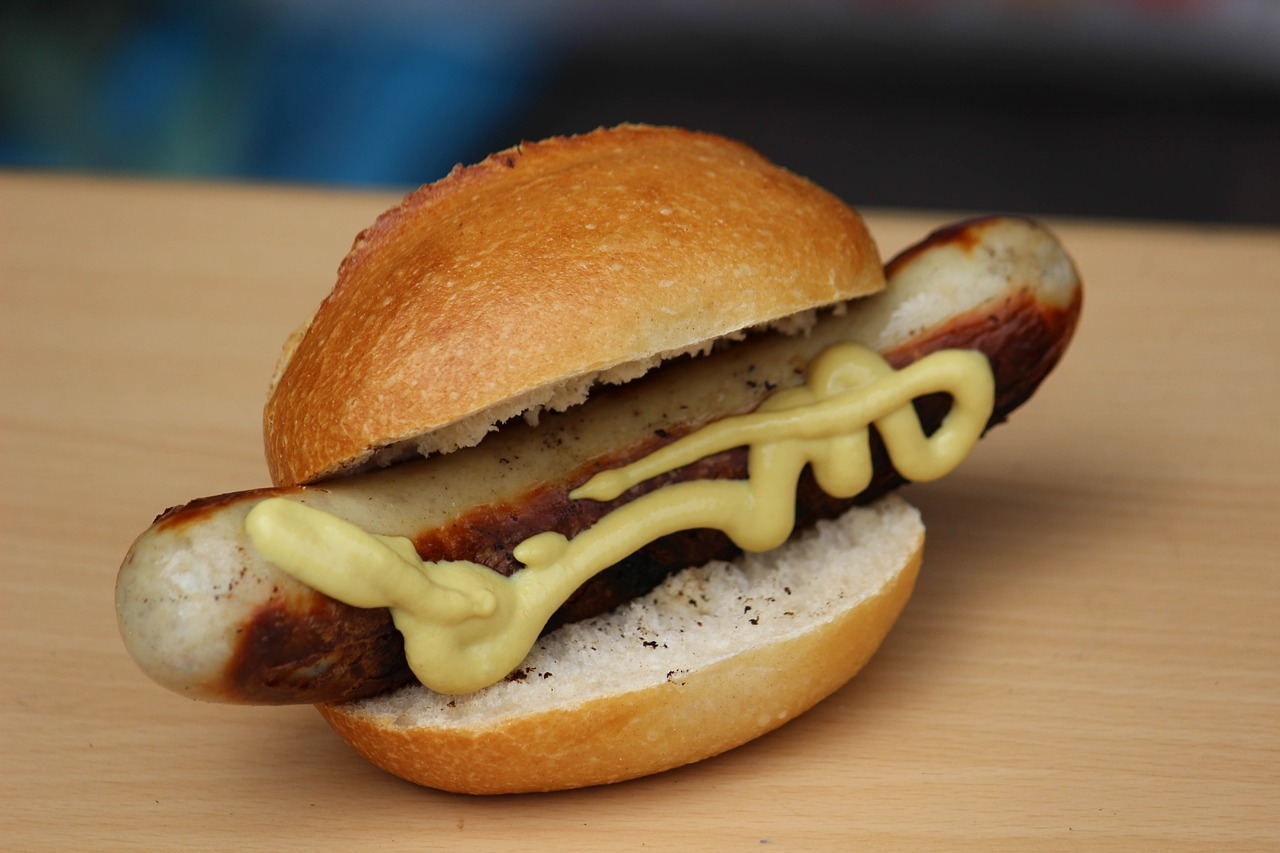
\includegraphics[width=0.5\textwidth]{images/bratwurst.jpg}
  \caption{Stock image of a~Bratwurst}
  \label{fig:wurst}
\end{figure}

The \texttt{figure} environment in Figure~\ref{fig:wurst} works just like
\texttt{table} (i.\,e.\ it's position is decided by \LaTeX).

\section{Footnotes}

Look down\footnote{
  \label{fn:my-footnote}
  Look, I'm at the bottom and all numbered well and stuff.
}.
Can you see Footnote~\ref{fn:my-footnote}?\footnote{
  Of course you can.
}

\section{Citations}

You can cite \citet{smith:2023} in-line, or you can just add parenthetical
citations \citep{muellerlapinsky:1986} to your text.
Also, you can add page numbers to your citations \citep[13--14]{actonetal:1997}
or additional labels \citep[cf.][54]{glargh:2030}.

\emph{Fun fact 1:}
You can easily create your own bibliography style by running \texttt{latex
makebst} on the command-line and answering a~bunch of questions.

\emph{Fun fact 2:}
I~already made a~bibliography style -- two, in fact -- \texttt{bibstyle-en.bst}
for English and \texttt{bibstyle-de.bst} for German.\footnote{%
  I.\,e.\ no Oxford comma, \& instead of the word \emph{and}, and other stuff
  I~don't remember.
}
If you want to use them for your stuff, go ahead.

\section{References}
\bibliography{sources}

\end{document}
